\documentclass[protokol.tex]{subfiles}
\begin{document}
Pohyb kyvadla byl měřen pomocí automatického měřiče vzdálenosti a doby kmitů byly poté vyhodnoceny pomocí počítače. Jelikož časový krok při měření činil 0,05 s, byla tato hodnota také zvolena jako chyba měřidla.
\begin{table}[H] 
\centering
\setlength{\tabcolsep}{15pt}
\begin{tabular}{cccccccc}																													\toprule
						&	1		&	2		&	3		&	průměr	&	$\sigma_{stat}$	&	$\sigma_{\text{měř}}$	&	$\sigma_{abs}$	\\	\midrule
$5 T_0 [\si{\second}]$	&	9,40	&	9,40	&	9,40	&	9,40	&	0,00			&	0,05					&	0,05			\\
$T_0 [\si{\second}]$	&	1,88	&	1,88	&	1,88	&	1,88	&	0,00			&	0,01					&	0,01			\\	\bottomrule
\end{tabular}
\caption{Naměřené hodnoty $T_0$}
\label{tab:t_0}
\end{table}

\begin{table}[H] 
\centering
\setlength{\tabcolsep}{15pt}
\begin{tabular}{cccccccc}																														\toprule
						&	1		&	2		&	3		&	průměr	&	$\sigma_{stat}$	&	$\sigma_{\text{měř}}$	&	$\sigma_{abs}$	\\	\midrule
$6 T_1   [\si{\second}]$&	11,20	&	11,25	&	11,20	&	11,22	&	0,017			&	0,05					&	0,05			\\	
$  T_1   [\si{\second}]$&	1,87	&	1,88	&	1,87	&	1,87	&	0,003			&	0,01					&	0,01			\\	\midrule
$6 T_2   [\si{\second}]$&	10,80	&	10,70	&	10,75	&	10,75	&	0,029			&	0,05					&	0,06			\\	
$  T_2   [\si{\second}]$&	1,80	&	1,78	&	1,79	&	1,79	&	0,005			&	0,01					&	0,01			\\	\midrule
$5 T_3   [\si{\second}]$&	9,20	&	9,20	&	9,20	&	9,20	&	0,000			&	0,05					&	0,05			\\	
$  T_3   [\si{\second}]$&	1,84	&	1,84	&	1,84	&	1,84	&	0,000			&	0,01					&	0,01			\\	\midrule
$  T_s/2 [\si{\second}]$&	42,10	&	41,25	&	41,10	&	41,48	&	0,311			&	0,05					&	0,32			\\	
$  T_s   [\si{\second}]$&   84.20   &   82.50   &   82.20   &   82.97   &   0.623           &   0.10                    &   0.63            \\  \bottomrule

\end{tabular}
\caption{Naměřené hodnoty pro slabší pružinu}
\label{tab:t_slabsi}
\end{table}

\begin{table}[H] 
\centering
\setlength{\tabcolsep}{15pt}
\begin{tabular}{cccccccc}																														\toprule
						&	1		&	2		&	3		&	průměr	&	$\sigma_{stat}$	&	$\sigma_{\text{měř}}$	&	$\sigma_{abs}$	\\	\midrule
$6 T_1   [\si{\second}]$&	11,20	&	11,25	&	11,20	&	11,22	&	0,017			&	0,05					&	0,05			\\	
$  T_1   [\si{\second}]$&	1,87	&	1,88	&	1,87	&	1,87	&	0,003			&	0,01					&	0,01			\\	\midrule
$6 T_2   [\si{\second}]$&	10,40	&	10,35	&	10,35	&	10,37	&	0,017			&	0,05					&	0,05			\\	
$  T_2   [\si{\second}]$&	1,73	&	1,73	&	1,73	&	1,73	&	0,003			&	0,01					&	0,01			\\	\midrule
$5 T_3   [\si{\second}]$&	7,20	&	7,25	&	7,25	&	7,23	&	0,017			&	0,05					&	0,05			\\	
$  T_3   [\si{\second}]$&	1,80	&	1,81	&	1,81	&	1,81	&	0,004			&	0,01					&	0,01			\\	\midrule
$  T_s/2 [\si{\second}]$&	22,10	&	21,50	&	21,95	&	21,85	&	0,180			&	0,05					&	0,19			\\	
$  T_s   [\si{\second}]$&   44.20	&	43.00	&	43.90	&	43.70	&	0.361			&	0.10					&	0.37			\\	\bottomrule

\end{tabular}


\caption{Naměřené hodnoty pro silnější pružinu}
\label{tab:t_silnejsi}
\end{table}

Následující tabulka obsahuje měření kmitů kyvadel se shodnou a protilehlou fází pro několik vzdáleností pružiny od závěsu kyvadel. Vzdálenost $l$ byla měřena pásovým měřidlem, jedná se o vzdálenost od dolní hrany závěsu kyvadla po vrchní hranu úchytu pružiny.
\begin{table}[H] 
\centering
\setlength{\tabcolsep}{15pt}
\begin{tabular}{cccccccc}																																		\toprule
$l [\si{\milli\metre}]$	&							&	1		&	2		&	průměr	&	$\sigma_{stat}$	&	$\sigma_{\text{měř}}$	&	$\sigma_{abs}$	\\	\midrule
266						&	$6 T_1 [\si{\second}]$	&	11,20	&	11,20	&	11,20	&	0,000			&	0,05					&	0,05			\\	
						&	$  T_1 [\si{\second}]$	&	1,87	&	1,87	&	1,87	&	0,000			&	0,01					&	0,01			\\
						&	$6 T_2 [\si{\second}]$	&	10,25	&	10,20	&	10,23	&	0,025			&	0,05					&	0,06			\\
						&	$  T_2 [\si{\second}]$	&	1,71	&	1,70	&	1,70	&	0,004			&	0,01					&	0,01			\\	\midrule
247						&	$6 T_1 [\si{\second}]$	&	11,20	&	11,20	&	11,20	&	0,000			&	0,05					&	0,05			\\
						&	$  T_1 [\si{\second}]$	&	1,87	&	1,87	&	1,87	&	0,000			&	0,01					&	0,01			\\
						&	$6 T_2 [\si{\second}]$	&	10,30	&	10,55	&	10,43	&	0,125			&	0,05					&	0,13			\\
						&	$  T_2 [\si{\second}]$	&	1,72	&	1,76	&	1,74	&	0,021			&	0,01					&	0,02			\\	\midrule
218						&	$6 T_1 [\si{\second}]$	&	11,20	&	11,25	&	11,23	&	0,025			&	0,05					&	0,06			\\
						&	$  T_1 [\si{\second}]$	&	1,87	&	1,88	&	1,87	&	0,004			&	0,01					&	0,01			\\
						&	$6 T_2 [\si{\second}]$	&	10,50	&	10,50	&	10,50	&	0,000			&	0,05					&	0,05			\\
						&	$  T_2 [\si{\second}]$	&	1,75	&	1,75	&	1,75	&	0,000			&	0,01					&	0,01			\\	\midrule
195						&	$6 T_1 [\si{\second}]$	&	11,20	&	11,20	&	11,20	&	0,000			&	0,05					&	0,05			\\
						&	$  T_1 [\si{\second}]$	&	1,87	&	1,87	&	1,87	&	0,000			&	0,01					&	0,01			\\
						&	$6 T_2 [\si{\second}]$	&	10,65	&	10,55	&	10,60	&	0,050			&	0,05					&	0,07			\\
						&	$  T_2 [\si{\second}]$	&	1,78	&	1,76	&	1,77	&	0,008			&	0,01					&	0,01			\\	\midrule
173						&	$6 T_1 [\si{\second}]$	&	11,25	&	11,30	&	11,28	&	0,025			&	0,05					&	0,06			\\
						&	$  T_1 [\si{\second}]$	&	1,88	&	1,88	&	1,88	&	0,004			&	0,01					&	0,01			\\
						&	$6 T_2 [\si{\second}]$	&	10,65	&	10,70	&	10,68	&	0,025			&	0,05					&	0,06			\\
						&	$  T_2 [\si{\second}]$	&	1,78	&	1,78	&	1,78	&	0,004			&	0,01					&	0,01			\\	\bottomrule

\end{tabular}
\caption{Závislost dob kmitů na poloze pružiny}
\label{tab:t_vazba}
\end{table}

\subsection*{Úkol 1}
Z tabulky \ref{tab:t_0} vyčteme 
$$ T_0 = (1,88 \pm 0,01) \ \si{\second}. $$

\subsection*{Úkol 2}
Z tabulky \ref{tab:t_slabsi} zjistíme hodnoty pro slabší pružinu
$$T_{sl_1} = (1,87 \pm 0,01) \ \si{\second},$$
$$T_{sl_2} = (1,79 \pm 0,01) \ \si{\second},$$
$$T_{sl_3} = (1,84 \pm 0,01) \ \si{\second},$$
$$T_{sl_4} = (41,48 \pm 0,32) \ \si{\second}$$
a z tabulky \ref{tab:t_silnejsi} pak
$$T_{si_1} = (1,87 \pm 0,01) \ \si{\second},$$
$$T_{si_2} = (1,73 \pm 0,01) \ \si{\second},$$
$$T_{si_3} = (1,81 \pm 0,01) \ \si{\second},$$
$$T_{si_4} = (21,85 \pm 0,19) \ \si{\second}.$$

\subsection*{Úkol 3}
Dosazením hodnot z tabulky \ref{tab:t_slabsi} a \ref{tab:t_silnejsi} do \eqref{eq:omega} dostaneme
$$ \omega_{sl_1} = (3,361 \pm 0,016) \ \si{\per\second}, $$
$$ \omega_{sl_2} = (3,507 \pm 0,019) \ \si{\per\second}, $$
$$ \omega_{sl_3} = (3,415 \pm 0,019) \ \si{\per\second}, $$
$$ \omega_{sl_4} = (0,076 \pm 0,001) \ \si{\per\second}, $$
$$ \omega_{si_1} = (3,361 \pm 0,016) \ \si{\per\second}, $$
$$ \omega_{si_2} = (3,637 \pm 0,019) \ \si{\per\second}, $$
$$ \omega_{si_3} = (3,475 \pm 0,025) \ \si{\per\second}, $$
$$ \omega_{si_4} = (0,144 \pm 0,001) \ \si{\per\second}. $$

Použitím vztahu \eqref{eq:omega_3} a \eqref{eq:omega_4} získáme
$$ \omega_{sl_3} = (3,434 \pm 0,012) \ \si{\per\second}, $$
$$ \omega_{sl_4} = (0,073 \pm 0,012) \ \si{\per\second}, $$
$$ \omega_{si_3} = (3,499 \pm 0,012) \ \si{\per\second}, $$
$$ \omega_{si_4} = (0,138 \pm 0,012) \ \si{\per\second}. $$

\subsection*{Úkol 4}
Podle vztahu \eqref{eq:stupen_vazby} dostaneme stupeň vazby pro slabší pružinu
$$ \kappa_{sl} = (0,042 \pm 0,007) $$
a silnější pružinu
$$ \kappa_{si} = (0,079 \pm 0,007). $$

\subsection*{Úkol 5}
Následující graf zobrazuje závislost $\kappa$ na $l$ pomocí údajů z tabulky \ref{tab:t_vazba}. Je proložen kvadratickým fitem.
\begin{figure}[H]
\centering
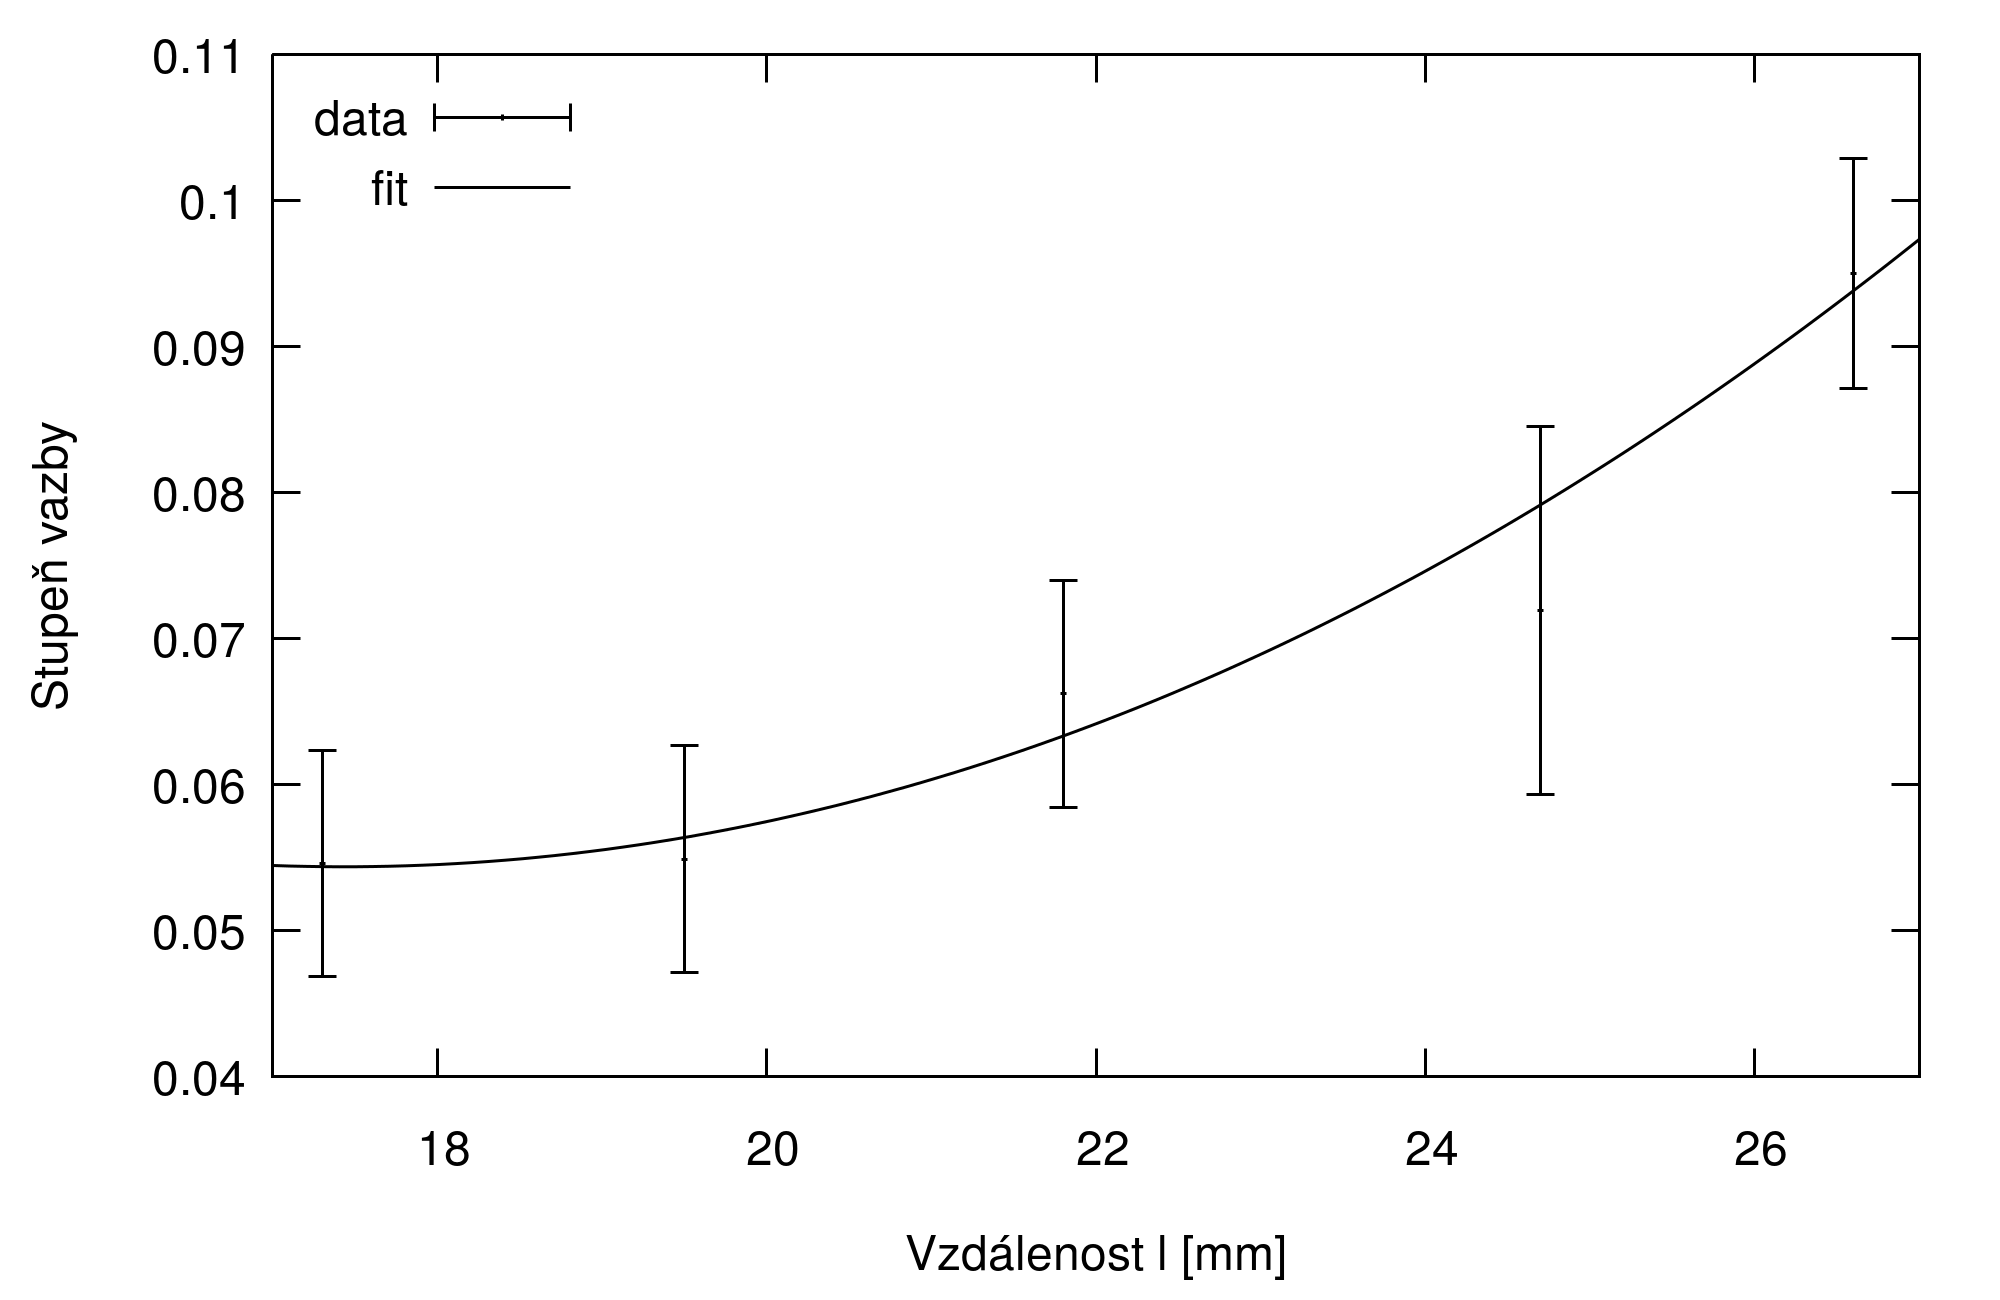
\includegraphics[resolution=350]{plot/graf}
\caption{Graf závislosti stupně vazby na vzdálenosti $l$}
\end{figure}
\end{document}
